\section{CMS Datasets} \label{section:higgs_data}

\subsection{Collision Datasets}
For the purpose of our search we use 35.9 fb$^{-1}$ of CMS collisions data collected over the course of 2016 datataking campaign. The full list of the datasets used is presented in the table~\ref{table:higgs_data_collisiondatasets}. The choice of SingleMuon stream (over DoubleMuon) is dictated by having intrinsically higher efficiency of triggering a single muon rather than two muons per a given event.
\begin{table}
    \caption{Datasets for proton-proton collisions recorded at $\sqrt{s}=13$~TeV by CMS at LHC in 2016.}
    \label{table:higgs_data_collisiondatasets}
    \begin{center}
        \begin{tabular}{ l  c}
            \hline
            Datasets & Int. Luminosity (fb$^{-1}$)\\
            \hline
            {/SingleMuon/Run2016B-03Feb2017\_ver2-v2/MINIAOD} & 5.788\\
            {/SingleMuon/Run2016C-03Feb2017-v1/MINIAOD} & 2.573\\
            {/SingleMuon/Run2016D-03Feb2017-v1/MINIAOD} & 4.248\\
            {/SingleMuon/Run2016E-03Feb2017-v1/MINIAOD} & 4.009\\
            {/SingleMuon/Run2016F-03Feb2017-v1/MINIAOD} & 3.102\\
            {/SingleMuon/Run2016G-03Feb2017-v1/MINIAOD} & 7.540\\
            {/SingleMuon/Run2016H-03Feb2017\_ver2(3)-v1/MINIAOD} & 8.606\\
            \hline
        \end{tabular}
    \end{center}
\end{table}

\subsection{Monte Carlo Datasets}
For the Standard Model Higgs Boson Signal, we use samples with three different hypothetical Higgs Boson masses. Since we are performing a search and are leaving the mass floating, we need a way to probe various hypotheses. Using three mass points (samples) we model parameters of each provided mass hypothesis and further perform interpolation to deduce the parameters for any mass point that falls within our range. Table~\ref{table:higgs_data_signaldatasets} provides a summary of CMS signal datasets used along with cross-section of each production process.
\begin{table}
    \caption{Standard Model 125 GeV Higgs Boson Signal Datasets for 13 TeV. Dataset names for 120/130 GeV are omitted for brevity. Moriond 2017 conditions are used (omitted the conditions specification for brevity).}
    \label{table:higgs_data_signaldatasets}
    \begin{center}
        \begin{tabular}{ l  c}
            \hline
            Datasets & $\sigma$ (pb)\\
            \hline
            {/GluGlu\_HToMuMu\_M125\_13TeV\_powheg\_pythia8} & 48.58\\
            {/VBF\_HToMuMu\_M125\_13TeV\_powheg\_pythia8} & 3.782\\
            {/WMinusH\_HToMuMu\_M125\_13TeV\_powheg\_pythia8} & 0.5331\\
            {/WPlusH\_HToMuMu\_M125\_13TeV\_powheg\_pythia8} & 0.851\\
            {/ZH\_HToMuMu\_M125\_13TeV\_powheg\_pythia8} & 0.8839 \\
            \hline
        \end{tabular}
    \end{center}
\end{table}
The Higgs signal production processes considered in this search are gluon
fusion (ggH), vector boson fusion (VBF), Higgsstrahlung (VH). Production in
association with top quarks (\ttH) has been generated privately. The Higgs MC samples are generated using {\sc POWHEG}~\cite{Nason:2004rx}.
\begin{table}[!h]
    \caption{Background Datasets. Moriond 2017 conditios have been used (omitted the conditions specification for brevity).}
    \label{table:higgs_data_backgrounddatasets}
    \begin{center}
        \begin{tabular}{ l  c}
            \hline
            Dataset & $\sigma$ (pb)\\
            \hline
            /DYJetsToLL\_M-50\_TuneCUETP8M1\_13TeV-amcatnloFXFX-pythia8 & 5765\\
            /ST\_tW\_top\_5f\_NoFullyHadronicDecays\_13TeV-powheg\_TuneCUETP8M1 & 35.85\\
            /TTJets\_DiLept\_TuneCUETP8M1\_13TeV-madgraphMLM-pythia8 & 85.656\\
            /WJetsToLNu\_TuneCUETP8M1\_13TeV-amcatnloFXFX-pythia8 & 61526.7\\
            /WWTo2L2Nu\_13TeV-powheg-herwigpp & 10.481\\
            /WZTo3LNu\_TuneCUETP8M1\_13TeV-amcatnloFXFX-pythia8 & 4.712\\
            \hline
        \end{tabular}
    \end{center}
\end{table}

Table~\ref{table:higgs_data_backgrounddatasets} provides a summary of the most dominant contributions among the background processes. Given that we use data-driven approach for our search, background samples are not used in any of the statistical modeling. However, the primary use of background datasets is to compare various kinematic variable distributions from data and theoretical predictions in section~\ref{section:higgs_results}. Moreover, as it will be clarified in section~\ref{section:higgs_categorization}, depending on the categorization technique used background samples can be used for training a binary classification algorithm for the purpose of signal discrimination.

Single top samples are generated with {\sc POWHEG}, while \ttbar samples and the multi-boson samples are generated either with {\sc madgrapgh}~\cite{Alwall:2011uj} or {amc@NLO (Next to Leading Order)}. Spin effects in multi boson processes are simulated using madspin. The parton shower and hadronization processes are modeled by the {\sc Pythia8} generator~\cite{Sjostrand:2007gs} with TuneCUETP8M1.

%The simulated pile up distribution is reweighted to match the observed
%distribution in data for all MC samples.

% \begin{table}[!h]
% \small
% \renewcommand{\arraystretch}{1.5}

% \begin{tabular}{|l||l|c|}
%     \hline \textbf{Dataset} & Run Range & Integrated Luminosity \\
%     \hline  &  & [fb$^{-1}$] \\
%     \hline
%         %% %% Fairly certain ver1-v1 is not used at all (no events in Golden JSON - AWB 13.05.16
%     %% \hline \url{/SingleMuon/Run2016B-03Feb2017_ver1-v1/MINIAOD} & \multirow{2}{*}{272007-275376} & \multirow{2}{*}{5.788} \\ \cline{1-1}
%     %% \url{/SingleMuon/Run2016B-03Feb2017_ver2-v2/MINIAOD} &  &  \\
%         \hline \url{/SingleMuon/Run2016B-03Feb2017_ver2-v2/MINIAOD} & 272007-275376 & 5.788 \\
%     \hline \url{/SingleMuon/Run2016C-03Feb2017-v1/MINIAOD}      & 275657-276283 & 2.573 \\
%     \hline \url{/SingleMuon/Run2016D-03Feb2017-v1/MINIAOD}      & 276315-276811 & 4.248 \\
%     \hline \url{/SingleMuon/Run2016E-03Feb2017-v1/MINIAOD}      & 276831-277420 & 4.009 \\
%     \hline \url{/SingleMuon/Run2016F-03Feb2017-v1/MINIAOD}      & 277772-278808 & 3.102 \\
%         \hline \url{/SingleMuon/Run2016G-03Feb2017-v1/MINIAOD}      & 278820-280385 & 7.540 \\
%     \hline \url{/SingleMuon/Run2016H-03Feb2017_ver2-v1/MINIAOD} & \multirow{2}{*}{280919-284044} & \multirow{2}{*}{8.606} \\ \cline{1-1}
%            \url{/SingleMuon/Run2016H-03Feb2017_ver3-v1/MINIAOD} &                                &                        \\
%     \hline                                                         %% Adds up to 35.866 - i.e. 35.9 fb^-1
%     \hline \multicolumn{3}{|l|}{\textbf{Luminosity mask: \url{Cert_271036-284044_13TeV_23Sep2016ReReco_Collisions16_JSON.txt}}}    \\
% \hline
% \end{tabular}

% \caption{Overview of the single muon data stream collected during the
% proton-proton collisions at $\sqrt{s}=13$~TeV by CMS at LHC in 2016.}
% \label{tab:datasets}
% \end{table}

% \newpage
% \begin{landscape}
% \begin{table}[p]
% \renewcommand{\arraystretch}{1.5}
% \tiny
% \begin{tabular}{|l||c|c|c|}
%   \hline \textbf{Higgs signal MC samples} & Events & Cross section [pb] & Xsec $\times$ BR [fb]  \\
%   %% From Yellow Report 4 (https://arxiv.org/abs/1610.07922), H --> mu-mu branching ratio at 125 GeV = 0.0002176
%   %% ggH = 48.58 pb, VBF = 3.7817 pb, W+H = 0.09426 pb, W-H = 0.05983 pb, ZH = 0.17762 pb, ttH = 0.5071 pb
%   \hline
%   \hline \url{/GluGlu_HToMuMu_M125_13TeV_powheg_pythia8/RunIISummer16MiniAODv2-PUMoriond17_80X_mcRun2_asymptotic_2016_TrancheIV_v6-v1/MINIAODSIM }  &  250000 & 48.58    & 10.571   \\
%   \hline \url{/VBF_HToMuMu_M125_13TeV_powheg_pythia8/RunIISummer16MiniAODv2-PUMoriond17_80X_mcRun2_asymptotic_2016_TrancheIV_v6-v1/MINIAODSIM }     &  249200 &  3.7817  & 0.8229   \\
%   \hline \url{/WPlusH_HToMuMu_M125_13TeV_powheg_pythia8/RunIISummer16MiniAODv2-PUMoriond17_80X_mcRun2_asymptotic_2016_TrancheIV_v6-v1/MINIAODSIM }  &  124547 &  0.09426 & 0.02051  \\
%   \hline \url{/WMinusH_HToMuMu_M125_13TeV_powheg_pythia8/RunIISummer16MiniAODv2-PUMoriond17_80X_mcRun2_asymptotic_2016_TrancheIV_v6-v1/MINIAODSIM } &  125000 &  0.05983 & 0.013019 \\
%   \hline \url{/ZH_HToMuMu_M125_13TeV_powheg_pythia8/RunIISummer16MiniAODv2-PUMoriond17_80X_mcRun2_asymptotic_2016_TrancheIV_v6-v1/MINIAODSIM }      &  249748 &  0.17762 & 0.03865  \\
%   %% \hline \url{/ttHToNonbb_M125_TuneCUETP8M2_ttHtranche3_13TeV-powheg-pythia8/RunIISummer16MiniAODv2-PUMoriond17_80X_mcRun2_asymptotic_2016_TrancheIV_v6-v1/MINIAODSIM } & 3981250 & 0.5071 & 0.11034 \\

% \hline
% \end{tabular}

% \caption{The Higgs signal MC samples were generated with {\sc POWHEG}
% while the parton shower and hadronization processes are modeled by the
% {\sc Phythia8} generator with TuneCUETP8M1.}
% \label{tab:SignalMC}
% \end{table}
% \end{landscape}

% \newpage
% \begin{landscape}
% \begin{table}[p]
% \tiny
% \renewcommand{\arraystretch}{1.2}
% \begin{tabular}{|l||c|c|}
%     \hline \textbf{Background MC} & Events & Cross Section [pb]  \\
%     \hline
%     \hline \multicolumn{3}{|c|}{\textbf{Drell--Yan}}  \\
%     \hline
%     \hline \url{/DYJetsToLL_M-50_TuneCUETP8M1_13TeV-amcatnloFXFX-pythia8/RunIISummer16MiniAODv2-PUMoriond17_80X_mcRun2_asymptotic_2016_TrancheIV_v6_ext2-v1/MINIAODSIM} &  122055388 & 5765  \\
%     \hline \url{/DYToLL_0J_13TeV-amcatnloFXFX-pythia8/RunIISummer16MiniAODv2-PUMoriond17_80X_mcRun2_asymptotic_2016_TrancheIV_v6_ext1-v1/MINIAODSIM} & 49579613  &  4754\\
%     %% \hline \url{/DYToLL_0J_13TeV-amcatnloFXFX-pythia8/RunIISummer16MiniAODv2-PUMoriond17_backup_80X_mcRun2_asymptotic_2016_TrancheIV_v6-v1/MINIAODSIM} & 44253240  &  4754    \\
%     \hline \url{/DYToLL_1J_13TeV-amcatnloFXFX-pythia8/RunIISummer16MiniAODv2-PUMoriond17_80X_mcRun2_asymptotic_2016_TrancheIV_v6_ext1-v1/MINIAODSIM} & 49902571  & 888.9 \\
%     %% \hline \url{/DYToLL_1J_13TeV-amcatnloFXFX-pythia8/RunIISummer16MiniAODv2-PUMoriond17_backup_80X_mcRun2_asymptotic_2016_TrancheIV_v6-v1/MINIAODSIM} & 41597712  & 888.9 \\
%     \hline \url{/DYToLL_2J_13TeV-amcatnloFXFX-pythia8/RunIISummer16MiniAODv2-PUMoriond17_80X_mcRun2_asymptotic_2016_TrancheIV_v6-v2/MINIAODSIM} & 42324802  & 348.8 \\
%     \hline \url{/DYToLL_2J_13TeV-amcatnloFXFX-pythia8/RunIISummer16MiniAODv2-PUMoriond17_80X_mcRun2_asymptotic_2016_TrancheIV_v6_ext1-v1/MINIAODSIM} & 47974554  & 348.8 \\
%     %% \hline \url{/DYJetsToLL_M-100to200_TuneCUETP8M1_13TeV-amcatnloFXFX-pythia8/RunIISummer16MiniAODv2-PUMoriond17_80X_mcRun2_asymptotic_2016_TrancheIV_v6_ext1-v1/MINIAODSIM} &  1083606 &  ??? \\
%     \hline
%     \hline \multicolumn{3}{|c|}{\textbf{SingleTop}}    \\
%     \hline
%     \hline \url{/ST_tW_top_5f_NoFullyHadronicDecays_13TeV-powheg_TuneCUETP8M1/RunIISummer16MiniAODv2-PUMoriond17_80X_mcRun2_asymptotic_2016_TrancheIV_v6-v1/MINIAODSIM} & 5372991  & 35.85 \\
%     \hline \url{/ST_tW_top_5f_NoFullyHadronicDecays_13TeV-powheg_TuneCUETP8M1/RunIISummer16MiniAODv2-PUMoriond17_80X_mcRun2_asymptotic_2016_TrancheIV_v6_ext1-v1/MINIAODSIM} & 3256650  & 35.85 \\
%     \hline \url{/ST_tW_antitop_5f_NoFullyHadronicDecays_13TeV-powheg_TuneCUETP8M1/RunIISummer16MiniAODv2-PUMoriond17_80X_mcRun2_asymptotic_2016_TrancheIV_v6-v1/MINIAODSIM} & 5425134  & 35.85 \\
%     \hline \url{/ST_tW_antitop_5f_NoFullyHadronicDecays_13TeV-powheg_TuneCUETP8M1/RunIISummer16MiniAODv2-PUMoriond17_80X_mcRun2_asymptotic_2016_TrancheIV_v6_ext1-v1/MINIAODSIM} & 3256407 & 35.85 \\
%     \hline
%     \hline \multicolumn{3}{|c|}{\textbf{TopPair}}    \\
%     \hline
%     \hline \url{/TTJets_DiLept_TuneCUETP8M1_13TeV-madgraphMLM-pythia8/RunIISummer16MiniAODv2-PUMoriond17_80X_mcRun2_asymptotic_2016_TrancheIV_v6-v1/MINIAODSIM} & 6094476 & 85.656 \\
%     \hline \url{/TTJets_DiLept_TuneCUETP8M1_13TeV-madgraphMLM-pythia8/RunIISummer16MiniAODv2-PUMoriond17_80X_mcRun2_asymptotic_2016_TrancheIV_v6_ext1-v1/MINIAODSIM} & 24350202  & 85.656 \\
%     \hline \url{/TTJets_Dilept_TuneCUETP8M2T4_13TeV-amcatnloFXFX-pythia8/RunIISummer16MiniAODv2-PUMoriond17_80X_mcRun2_asymptotic_2016_TrancheIV_v6-v1/MINIAODSIM} &  14529280 & 85.656  \\
%     \hline
%     \hline \multicolumn{3}{|c|}{\textbf{DiBoson}}    \\
%     \hline
%     \hline \url{/WWTo2L2Nu_13TeV-powheg/RunIISummer16MiniAODv2-PUMoriond17_80X_mcRun2_asymptotic_2016_TrancheIV_v6-v1/MINIAODSIM } & 1999000  & 12.46  \\
%     \hline \url{/WZTo3LNu_TuneCUETP8M1_13TeV-amcatnloFXFX-pythia8/RunIISummer16MiniAODv2-PUMoriond17_80X_mcRun2_asymptotic_2016_TrancheIV_v6-v1/MINIAODSIM} & 11887464  & 2.113 \\
%     \hline \url{/WZTo2L2Q_13TeV_amcatnloFXFX_madspin_pythia8/RunIISummer16MiniAODv2-PUMoriond17_80X_mcRun2_asymptotic_2016_TrancheIV_v6-v1/MINIAODSIM} & 26517272  &  4.409 \\
%     \hline \url{/ZZTo2L2Nu_13TeV_powheg_pythia8/RunIISummer16MiniAODv2-PUMoriond17_80X_mcRun2_asymptotic_2016_TrancheIV_v6-v1/MINIAODSIM} & 8842475  & 0.564  \\
%     \hline \url{/ZZTo2L2Q_13TeV_amcatnloFXFX_madspin_pythia8/RunIISummer16MiniAODv2-PUMoriond17_80X_mcRun2_asymptotic_2016_TrancheIV_v6-v1/MINIAODSIM} & 15345572  & 3.22 \\
%     \hline \url{/ZZTo4L_13TeV-amcatnloFXFX-pythia8/RunIISummer16MiniAODv2-PUMoriond17_80X_mcRun2_asymptotic_2016_TrancheIV_v6_ext1-v1/MINIAODSIM} &  10709784 & 1.212  \\
%     \hline
%     \hline \multicolumn{3}{|c|}{\textbf{TriBoson}}   \\
%     \hline
%     \hline \url{/WWW_4F_TuneCUETP8M1_13TeV-amcatnlo-pythia8/RunIISummer16MiniAODv2-PUMoriond17_80X_mcRun2_asymptotic_2016_TrancheIV_v6-v1/MINIAODSIM } & 240000   &     0.2086  \\
%     \hline \url{/WWZ_TuneCUETP8M1_13TeV-amcatnlo-pythia8/RunIISummer16MiniAODv2-PUMoriond17_80X_mcRun2_asymptotic_2016_TrancheIV_v6-v1/MINIAODSIM} & 250000  & 0.1651 \\
%     \hline \url{/WZZ_TuneCUETP8M1_13TeV-amcatnlo-pythia8/RunIISummer16MiniAODv2-PUMoriond17_80X_mcRun2_asymptotic_2016_TrancheIV_v6-v1/MINIAODSIM} & 246800  & 0.05565 \\
%     \hline \url{/ZZZ_TuneCUETP8M1_13TeV-amcatnlo-pythia8/RunIISummer16MiniAODv2-PUMoriond17_80X_mcRun2_asymptotic_2016_TrancheIV_v6-v1/MINIAODSIM} & 249237  & 0.01398 \\
%     \hline
%     \hline \multicolumn{3}{|c|}{\textbf{SingleTop+X}}    \\
%     \hline
%     \hline \url{/tZq_ll_4f_13TeV-amcatnlo-pythia8/RunIISummer16MiniAODv2-PUMoriond17_80X_mcRun2_asymptotic_2016_TrancheIV_v6_ext1-v1/MINIAODSIM } & 14509520  & 0.0758  \\
%     %\hline \url{/ST_tWll_5f_LO_13TeV-MadGraph-pythia8/RunIISummer16MiniAODv2-PUMoriond17_80X_mcRun2_asymptotic_2016_TrancheIV_v6-v1/MINIAODSIM} &  50000 & ??? \\
%     \hline
%     \hline \multicolumn{3}{|c|}{\textbf{Top pairs}}    \\
%     \hline
%     \hline \url{/TTWJetsToLNu_TuneCUETP8M1_13TeV-amcatnloFXFX-madspin-pythia8/RunIISummer16MiniAODv2-PUMoriond17_80X_mcRun2_asymptotic_2016_TrancheIV_v6_ext1-v3/MINIAODSIM     } & 2160168  & 0.2043 \\
%     \hline \url{/TTWJetsToLNu_TuneCUETP8M1_13TeV-amcatnloFXFX-madspin-pythia8/RunIISummer16MiniAODv2-PUMoriond17_80X_mcRun2_asymptotic_2016_TrancheIV_v6_ext2-v1/MINIAODSIM} & 3120397  & 0.2043 \\
%     \hline \url{/TTZToLLNuNu_M-10_TuneCUETP8M1_13TeV-amcatnlo-pythia8/RunIISummer16MiniAODv2-PUMoriond17_80X_mcRun2_asymptotic_2016_TrancheIV_v6_ext1-v1/MINIAODSIM} & 1992438  & 0.2529 \\

% \hline

% \end{tabular}

% \caption{The MC background processes samples were generated with {amc@NLO}.
% {\sc POWHEG} and {\sc madgrapgh}. Spin effects in multi boson processes are
% simulated using  {\sc madspin}. The parton shower and hadronization processes
%  are modeled by the {\sc Phythia8} generator with TuneCUETP8M1.}
% \label{tab:BkgMC}
% \end{table}
% \end{landscape}

%\subsection{Pileup Reweighting}
%\label{pu}

% Each MC samples is reweighted in order to match the pileup distribution in data, as centrally recommended using the ``minimum bias'' cross section of $69.2$mb $\pm5\%$.
% The value needs to be read as an effective minimum bias times efficiesies cross section with respect to what present in pythia8; large uncertainties are present in order to cover differences between the run period and the charge/neutral compenents.

% \begin{figure}[h!]
%     \centering
%     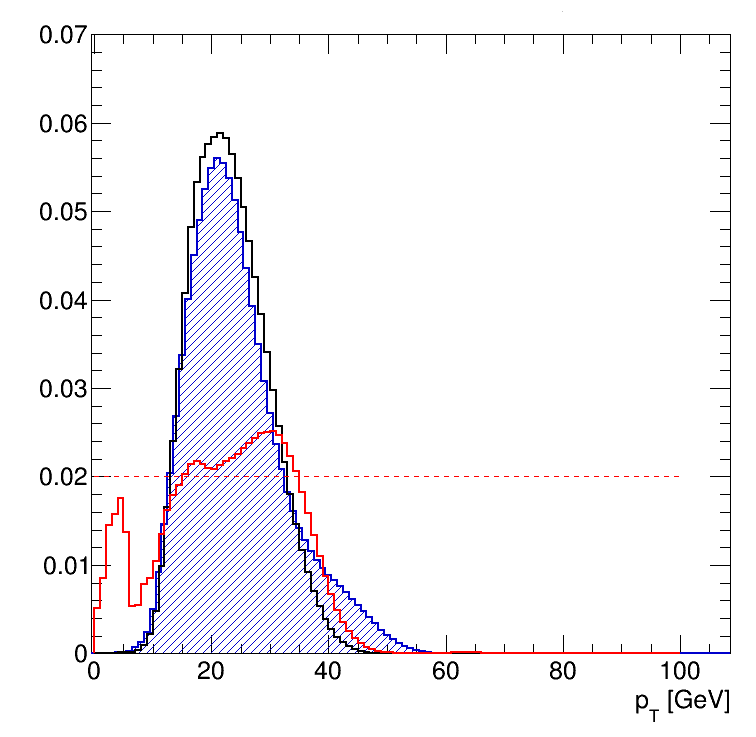
\includegraphics[width=0.49\textwidth]{figures/data_mc_samps/Pu-reweight2.png}
%     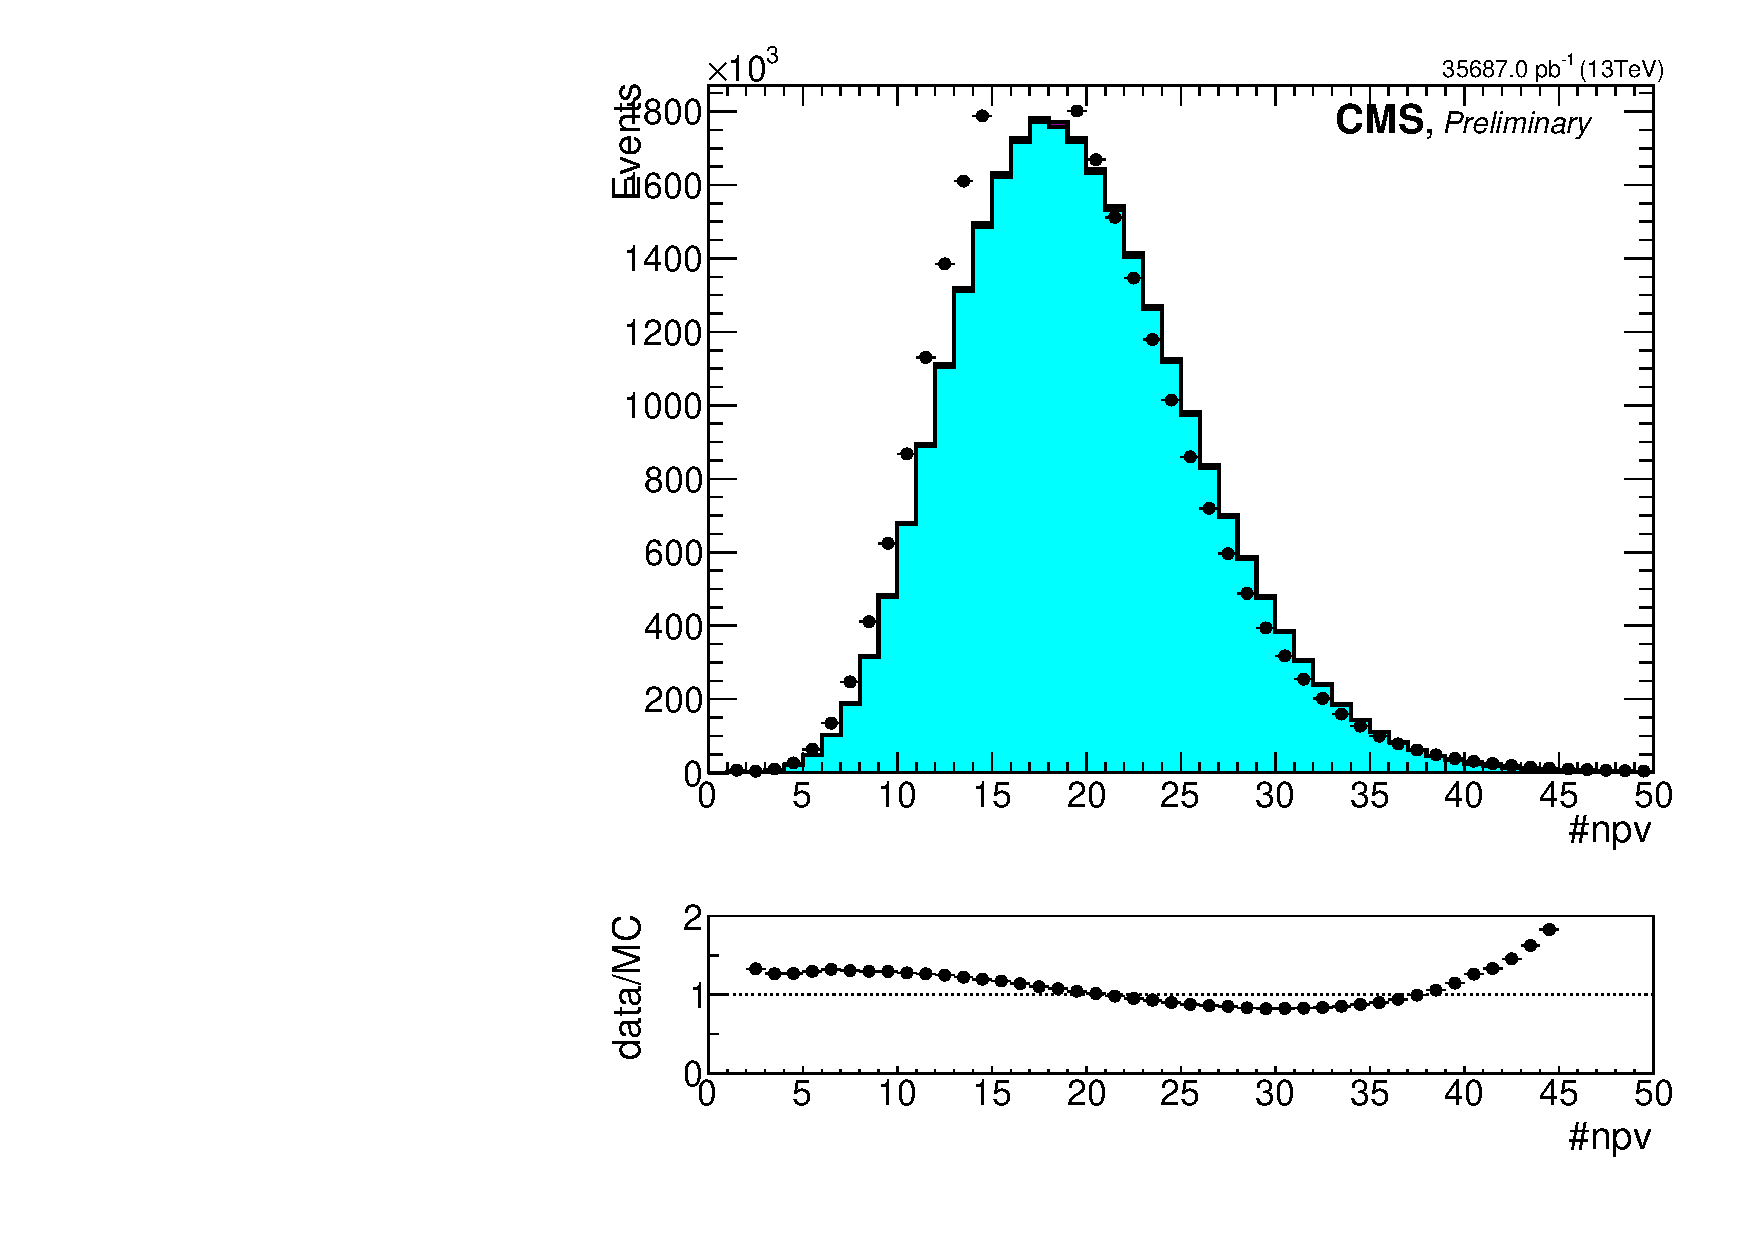
\includegraphics[width=0.49\textwidth]{figures/data_mc_samps/mmNpv_pileup69200.pdf}\\
%     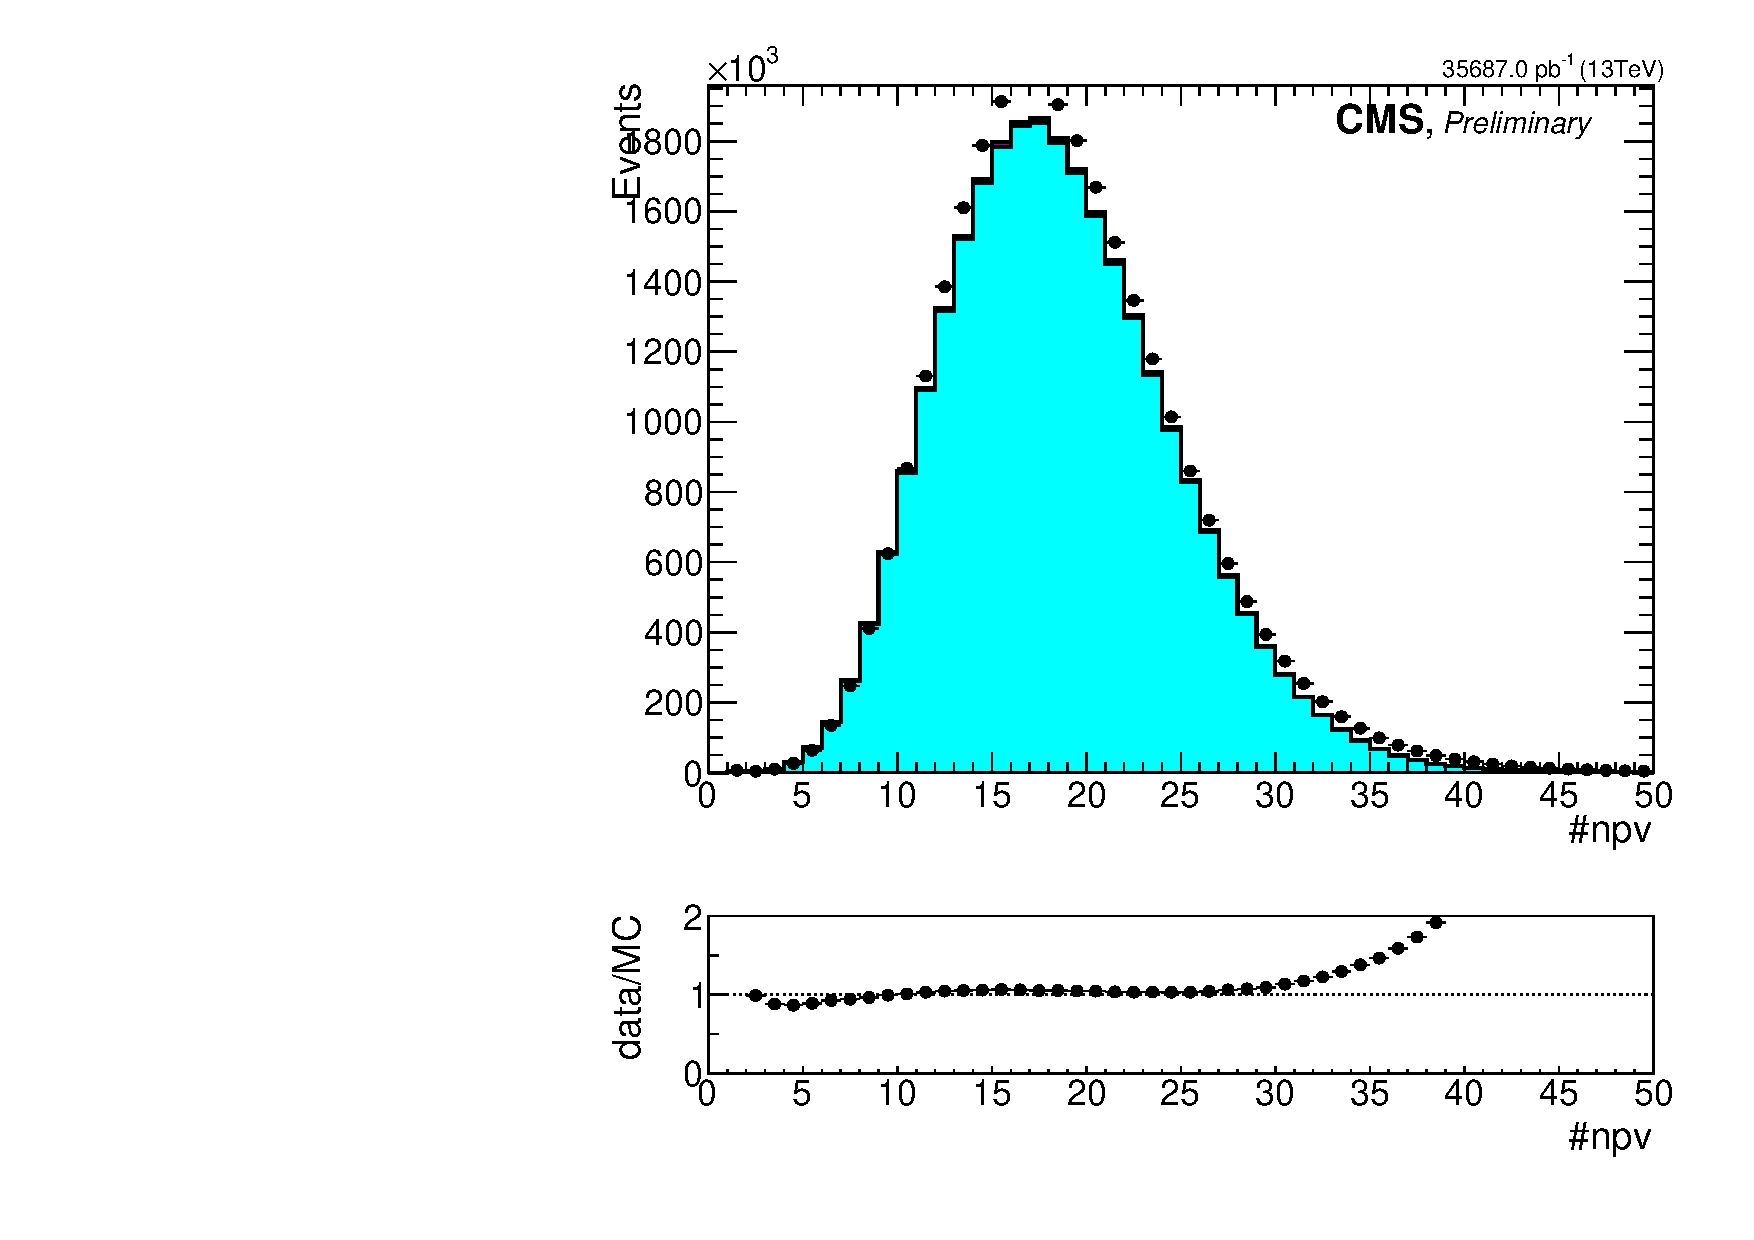
\includegraphics[width=0.49\textwidth]{figures/data_mc_samps/mmNpv_pileup65000.pdf}
%     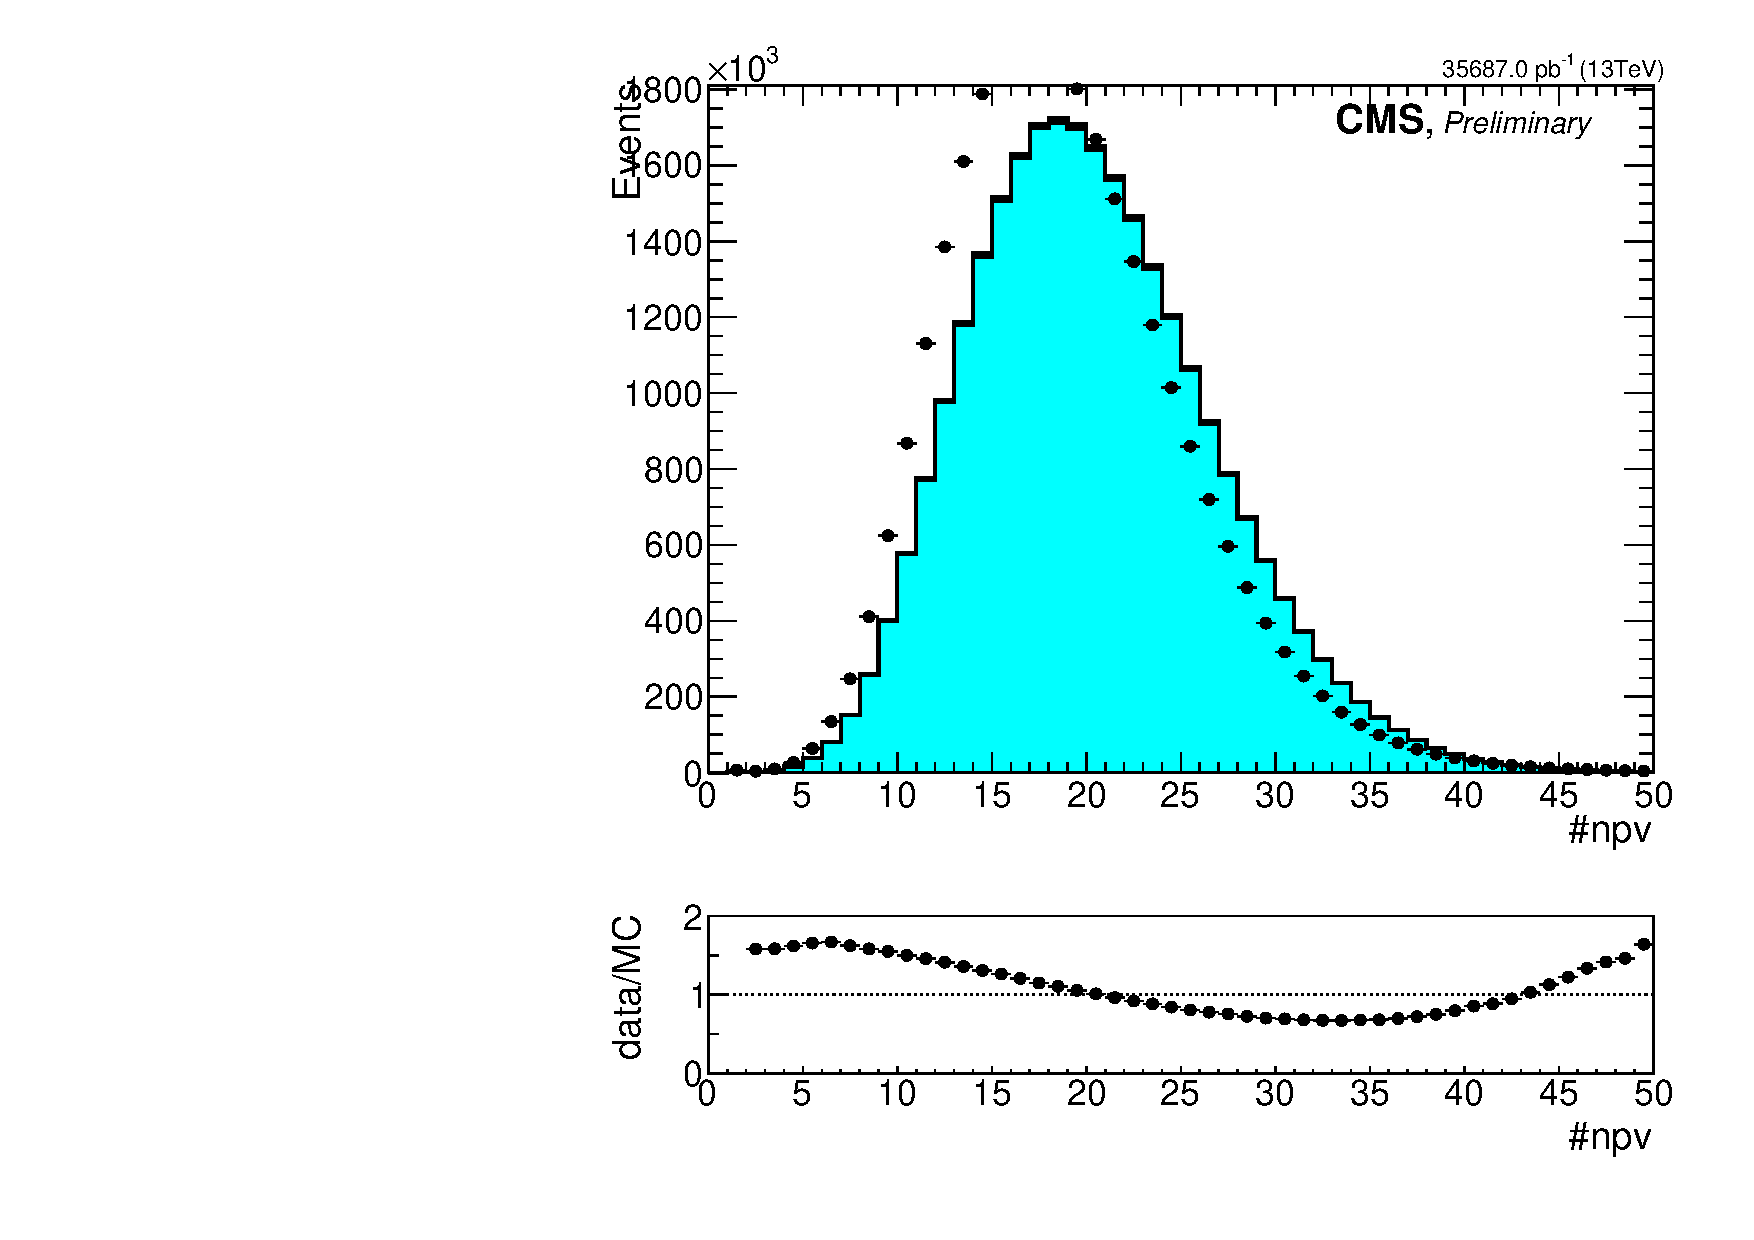
\includegraphics[width=0.49\textwidth]{figures/data_mc_samps/mmNpv_pileup72000.pdf}
%     \caption{Top Left. Pileup reweighting factors, data and MC truth pileup distributions. Top Right. agreement in the number of primary vertex variable after pu-reweighting. Bottom. agreement for the n.p.v. variables after $\pm1\sigma$ uncertainty in the pu-reweighting cress section.}
% \end{figure}



